% !TEX root = ../main.tex
\newpage
\section{Mean Field Reductions} \label{sec:MFRs}
\subsection{The Ott-Antonsen manifold}
The \textsl{mean-field reduction} (\MFR) is a theory that can predict the dynamics of the order parameter \eqref{eq:orderparameter}. In \cite{OttAntonsen2008, OttAntonsen2009, OttAntonsen2010} such a method was published for fully connected networks of indistinguishable oscillators with harmonic coupling. In \cite{Restrepo2014} the authors extended their work to include networks with arbitrary degree distributions, applied to the Kuramoto model. Later this analysis was extended to networks of the Theta Neuron model \cite{OttAntonsen2017}. We will now consider the limit $N \gg 1$ and formulate an exact \MFR for different types of networks, following the method in \cite{OttAntonsen2017}. \\

To simplify notation, the authors incorporate the network size in to $P$ so that $\sum_{\k \in \K} P(\k) = N$. To specify the probability of a link from a node of degree $\kacc$ to one of degree $\k$ we can define an assortativity function:
\begin{align}
a\left(\k_j \rightarrow \k_i \right) = 0 \leq \frac{k^{\rm{out}^{\prime}}_j k^{\rm{in}}_i}{N \kmean} \leq 1 \label{eq:assortativityfunction}
\end{align}
where we have chosen a neutral assortativity \cite{OttAntonsen2017}. \eqref{eq:assortativityfunction} is constrained so that the number of links in the network, $N \kmean$, remains constant \cite{Restrepo2014}:
\begin{align*}
\sum_{\kacc \in \K} \sum_{\k \in \K} P\left( \kacc \right) \: a\left(\kacc \rightarrow \k\right) P\left(\k\right) = N \kmean
\end{align*}
We can now assume that the state of all neurons can be represented by a probability density function $f(\theta, \eta | \k, t)$. Hence, the marginal distribution 
\begin{align*}
    \int_{\R} \int_{\T} f(\vartheta, \eta^{\prime} | \k, t) \mathop{d \vartheta} \mathop{d \eta^{\prime}} 
\end{align*}
gives the fraction of nodes of degree $\k$ with a phase in $\T$ at time $t$. Also, we assume $\eta_i$ do not change over time, so that $\int_{\T} f(\vartheta, \eta^{\prime} | \k, t) \: \mathop{d \vartheta}$ yields the excitability distribution $g(\eta | \k)$. \\

To describe the global synchronisation of the network of theta neurons \eqref{eq:thetaneuronnetwork} we have introduced the order parameter $Z(t)$\eqref{eq:orderparameter}. It is now hypothesized that $Z(t)$ can be approximated by a mean-field order parameter, defined by the continuum limit:
\begin{align}
\bar{Z}(t)= \frac{1}{N} \sum_{\k \in \K}P(\k) \int_{\R} \int_{\T} f\left(\vartheta, \eta^{\prime} | \k, t\right) e^{\ic \vartheta} \mathop{d \vartheta} \mathop{d \eta^{\prime}} \label{eq:meanfieldorderparameter}
\end{align}
Here, $f$ is constrained by a continuity equation, as the number of oscillators is conserved:
\begin{align}
\frac{\partial f}{\partial t}+\frac{\partial}{\partial \theta}\left(v_{\theta} f\right) = 0 \label{eq:transportequation}
\end{align}
with $v_{\theta}$ a continuum version of \eqref{eq:thetaneuronnetwork}:
\begin{align*}
v_{\theta} &= (1-\cos \theta)+(1+\cos \theta) \left[\eta + I(\k,t) \right]\\
I(\k,t) &= \frac{\kappa}{\kmean}\sum_{\kacc \in \K} P(\kacc ) \:a\left(\kacc \rightarrow \k \right) \times \left[ \int_{\R} \int_{\T} f\left(\vartheta, \eta^{\prime} | \kacc, t\right) \: a_{n} \left(1-\cos \vartheta\right)^{n} \mathop{d \vartheta} \mathop{d \eta^{\prime}} \right] &
\end{align*}
In \cite{OttAntonsen2008} it is shown that there exists a manifold of invariant probability densities for the continuity equation. The exact \MFR is obtained by expanding $f$ as a Fourier series, and expanding the pulse $\mathcal{P}_n$ using the binomial theorem. When assuming $\eta_i$ is distributed according to a Lorenz distribution:
\begin{align}
g(\eta |\k)=\frac{1}{\pi} \frac{\sigma(\k)}{(\eta-\eta_{0}(\k))^{2}+\sigma(\k)^{2}} \label{eq:Lorentzpdf}
\end{align}
the set of reduced equations then takes a particularly simple form, as \eqref{eq:meanfieldorderparameter} can be evaluated at the poles of $g$ using the Cauchy residue theorem for the integration of complex variables and we find a closed form expression. We can now capture the dynamics by $z(\k,t)$, the mean-field variable for nodes of degree $\k$:
\begin{align}
\frac{\partial z(\k, t)}{\partial t} &= -\ic \frac{(z(\k, t)-1)^{2}}{2} + \frac{(z(\k, t)+1)^{2}}{2} \cdot I(\k, t) \qquad z \in \C^{M_\k} \nonumber \\
I(\k, t) &= -\sigma(\k) + \ic \eta_{0}(\k) + \ic H_2(\k,t) \label{eq:OttAntonsenSystemFull} \\
H_2(\k,t) &= \frac{\kappa}{\kmean} \sum_{\kacc \in \K} P\left(\kacc\right) \: a\left(\kacc \rightarrow \k\right)  \left( 1 + \frac{z(\kacc, t)^2 + (z(\kacc, t)^c )^2}{6} - \frac{4}{3} \Re(z(\kacc, t)) \right) \nonumber
\end{align}
with $z^c$ the complex conjugate. $H$ is a legacy term and has been computed in \cite{Martens2020}.
The mean-field order parameter can now be expressed in terms of $z(\k,t)$. Using the constraints on $f$ and $g$ we can now solve \eqref{eq:meanfieldorderparameter} as:
\begin{align}
\bar{Z}(t) &= \frac{1}{N} \sum_{\k \in \K} P(\k) z(\k, t) \qquad \bar{Z} \in \C \label{eq:OttAntonsenMeanField}
\end{align}
which clearly reflects the network architecture through $P(\k)$, as in the limit, this is the number of neurons of degree $\k$ that are present in the network. The mean-field dynamics of the whole network are thus equal to a weighed average of the degree dynamics of each node with unique degree $\k \in \K$. 

We have now formulated the evolution on the invariant manifold by a reduced set of ordinary differential equations. The \MFR is computationally efficient, and in \cite{OttAntonsen2017} many methods for improving this efficiency further are treated.


\subsection{Simplifications for fixed-degree networks}
In the case of a fixed-degree network, every node has $\deg (\theta_i) = (\kmean, \kmean)$ so:
\begin{align*}
    \frac{1}{\kmean} \sum_{\kacc \in \K} P\left(\kacc\right) \: a\left(\kacc \rightarrow \k\right) = \frac{1}{\kmean} N \left( \frac{\kmean \kmean}{N \kmean} \right) = 1
\end{align*}
For any fixed-degree network, \cref{eq:OttAntonsenSystemFull,eq:OttAntonsenMeanField} reduce to a single complex differential equation:
\begin{align}
\dot{Z}(t)= -\ic \frac{(Z-1)^2}{2}+\frac{(Z+1)^2}{2} \left(-\sigma+ \ic\eta_{0}
+ \ic \kappa \left(1+\frac{Z^{2} + (Z^c)^{2} }{6} - \frac{4}{3} \Re(Z)\right)\right) \label{eq:MeanField}
\end{align}
This is an identical formulation as in \cite{Luke2013} and \cite{Martens2020}. For any fixed-degree network, the reduced system is thus a complex (two-dimensional) system with three bifurcation parameters $\eta_0, \sigma$ and $\kappa$, \cite{Luke2013, Martens2020}. We will start our analysis with \eqref{eq:MeanField}.\\

Three distinct macroscopic states can be identified. In the partially synchronous rest state (\PSR) we can observe in Figure \ref{fig:MFRPSR}, $Z(t)$ settles onto a stable node. Most neurons can be found in a resting state $\eta_0 + \sigma \lesssim 0$, and inhibit one another through $\kappa < 0$. Most neurons are therefore inactive, though some spiking neurons from the tail of $g$ are present but have a neglegible effect. \\

In Figure \ref{fig:MFRPSS} we can observe the partially synchronous spiking (\PSS) state, where we can see how $Z(t)$ settles onto a stable focus. This happens predominantly when $\eta_0 - \sigma \gtrsim 0$ and most neurons inherently spike, with the coupling being either excitatory or weakly inhibitory. Although most neurons are active, the network is partially synchronous and organized such that phase cancellation occurs by continuous spiking among the neurons.\\

Lastly, in the collective periodic wave state (\CPW) we can observe a limit cycle of the mean field, in Figure \ref{fig:MFRCPW}. Most neurons are active and inhibitory: $\eta_0 > 0$ and $\kappa < 0$. The collective oscillation emerges from the interplay between the neurons’ inherent tendency to spike and the strong suppressive network interaction. \CPW states are mediated through Hopf bifurcations and homoclinic bifurcations of $Z(t)$. We can also see the occurrence of a saddle-node bifurcation in the lower hand corner, for low $\sigma$. We will continue to study the \CPW due to its interesting properties.\\

A more detailed discussion of the different regimes and bifurcations can be found in \cite{Luke2013}.

% \textcolor{red}{QUESTION}: \textsl{I have worked on the analysis presented in \cite{Luke2013} to make my own figures on the bifurcations. However, I cannot seem to get them plotted. Should I continue on this?}

\begin{figure}[H]
\centering
\begin{subfigure}[b]{0.32\linewidth}
   \centering
  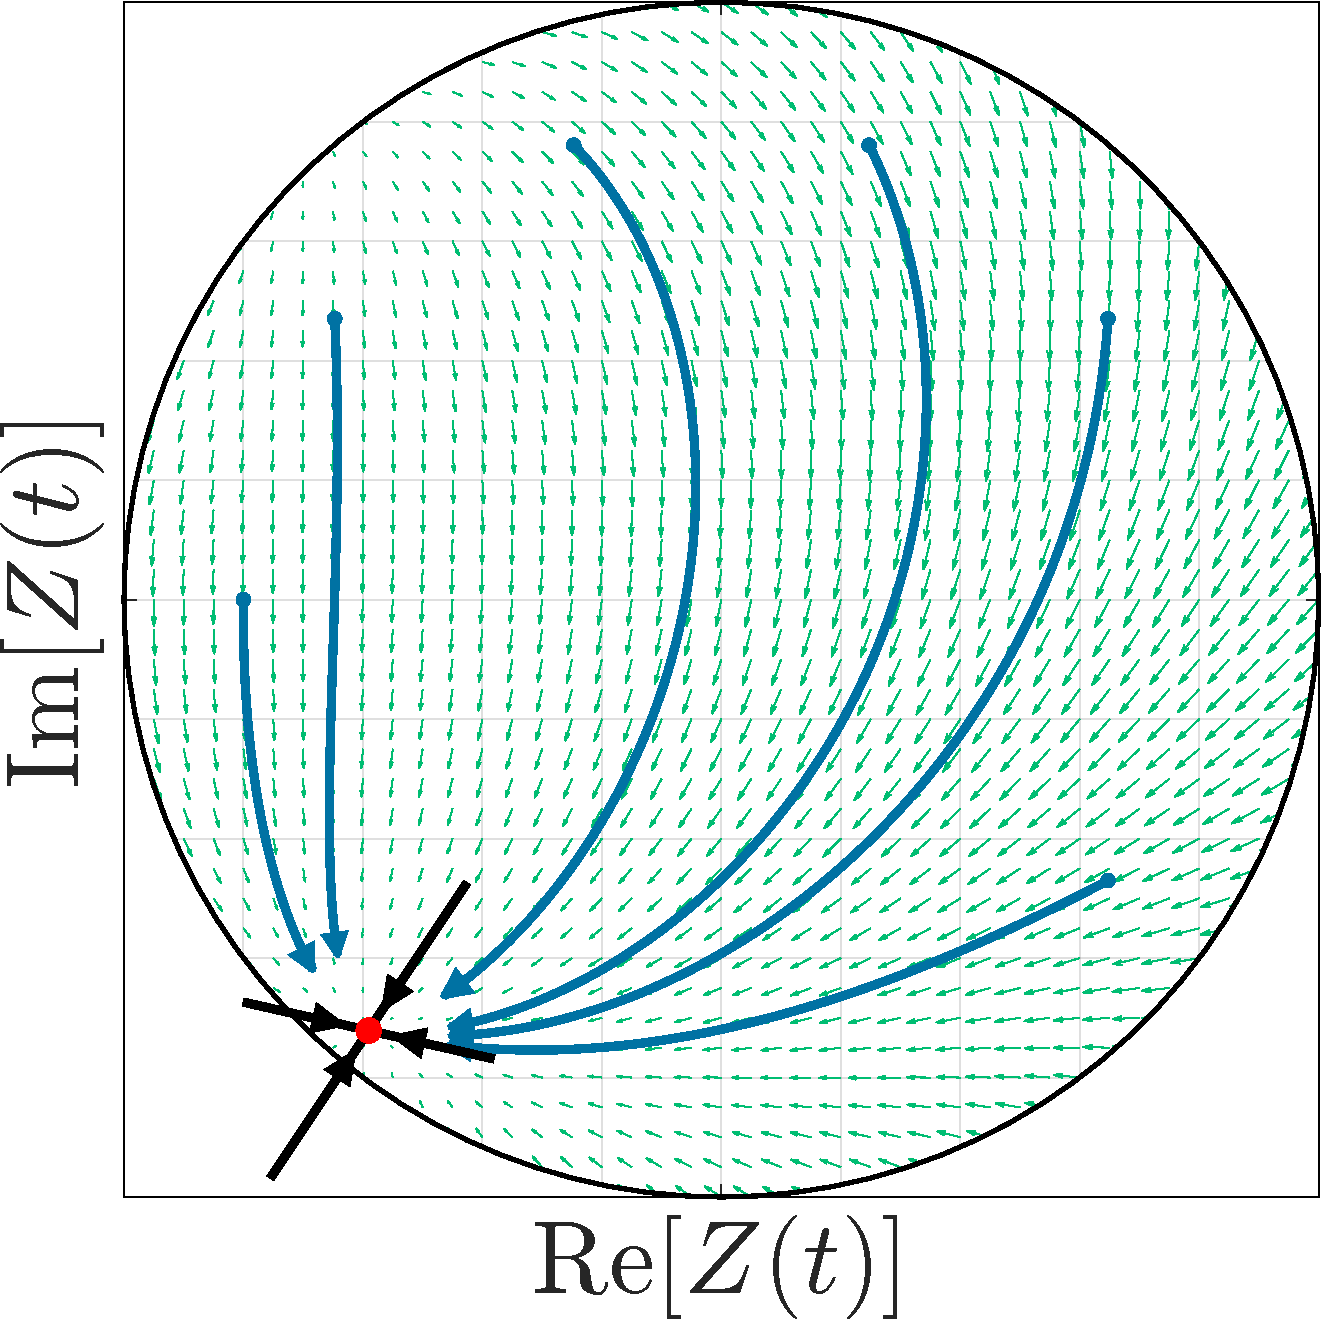
\includegraphics[width=\linewidth]{../Figures/PhaseSpace/MFRPSR.pdf}
   \caption{PSR state for $\eta_0 = -0.9, \sigma = 0.8$ and $\kappa= -2$. The mean field settles onto a stable node.}
   \label{fig:MFRPSR} 
\end{subfigure} \hfill
\begin{subfigure}[b]{0.32\linewidth}
   \centering
  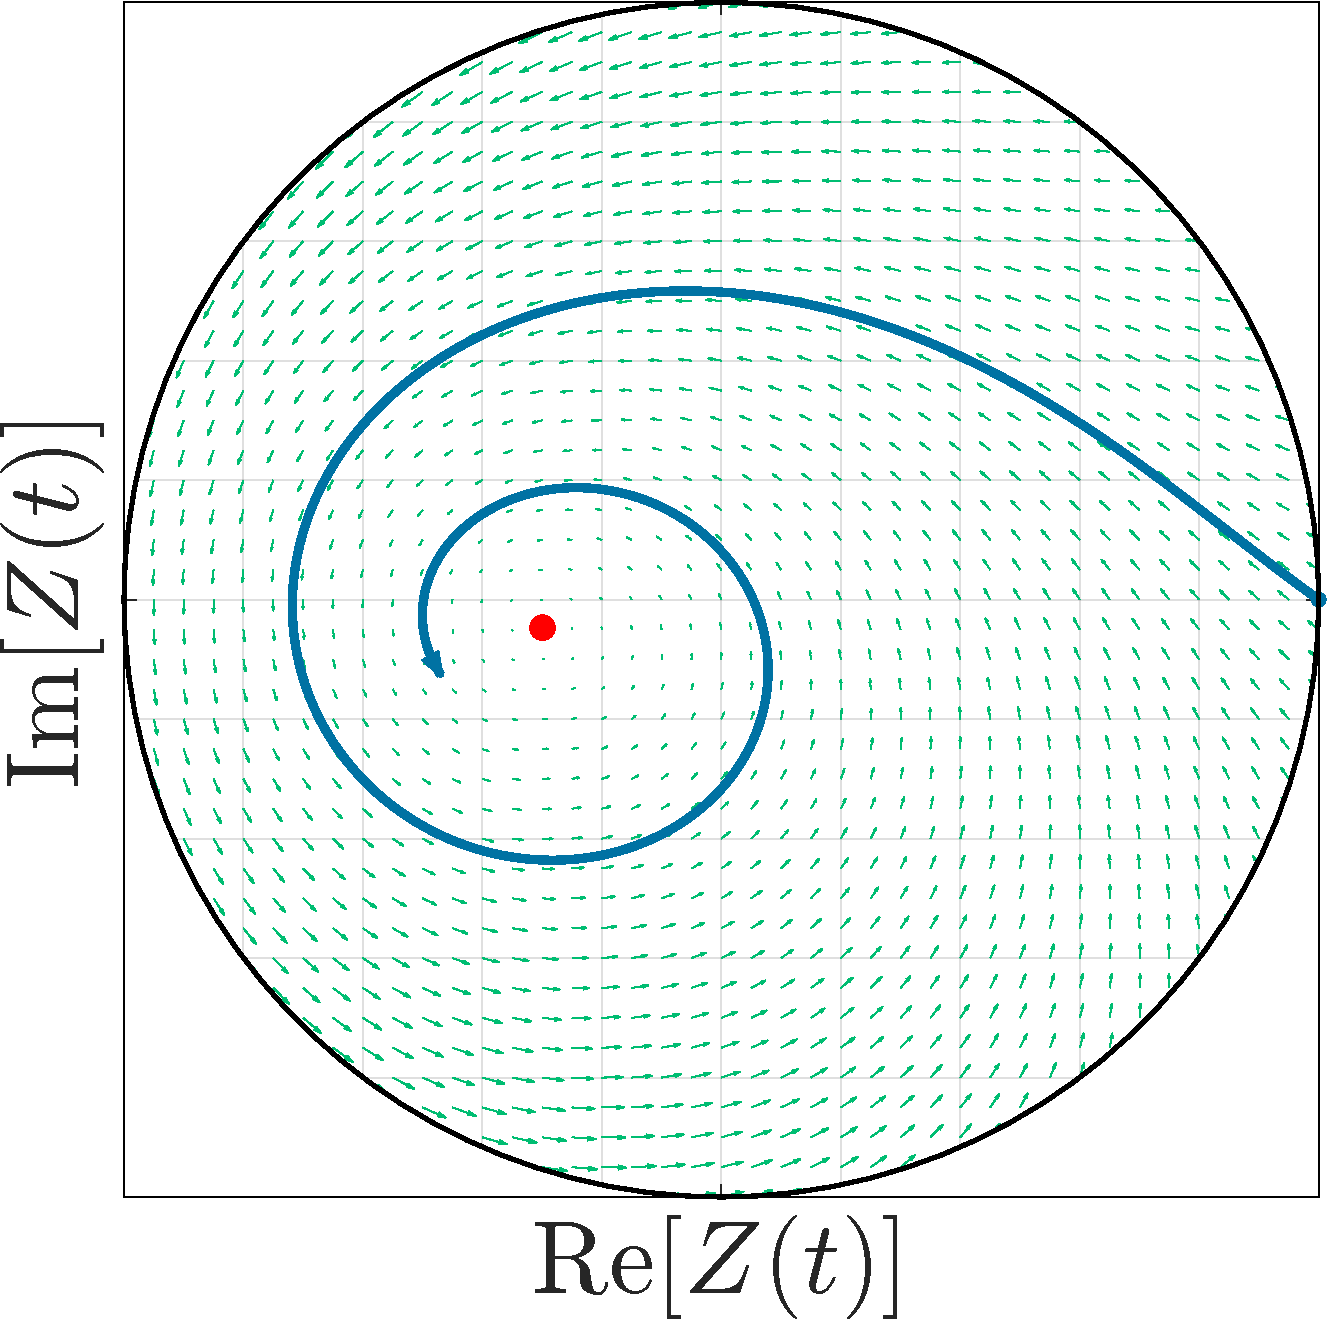
\includegraphics[width=\linewidth]{../Figures/PhaseSpace/MFRPSS.pdf}
   \caption{PSS state for $\eta_0 = 0.5, \sigma = 0.7$ and $\kappa= 2$. The mean field settles onto a stable focus.}
   \label{fig:MFRPSS}
\end{subfigure} \hfill
\begin{subfigure}[b]{0.32\linewidth}
   \centering
  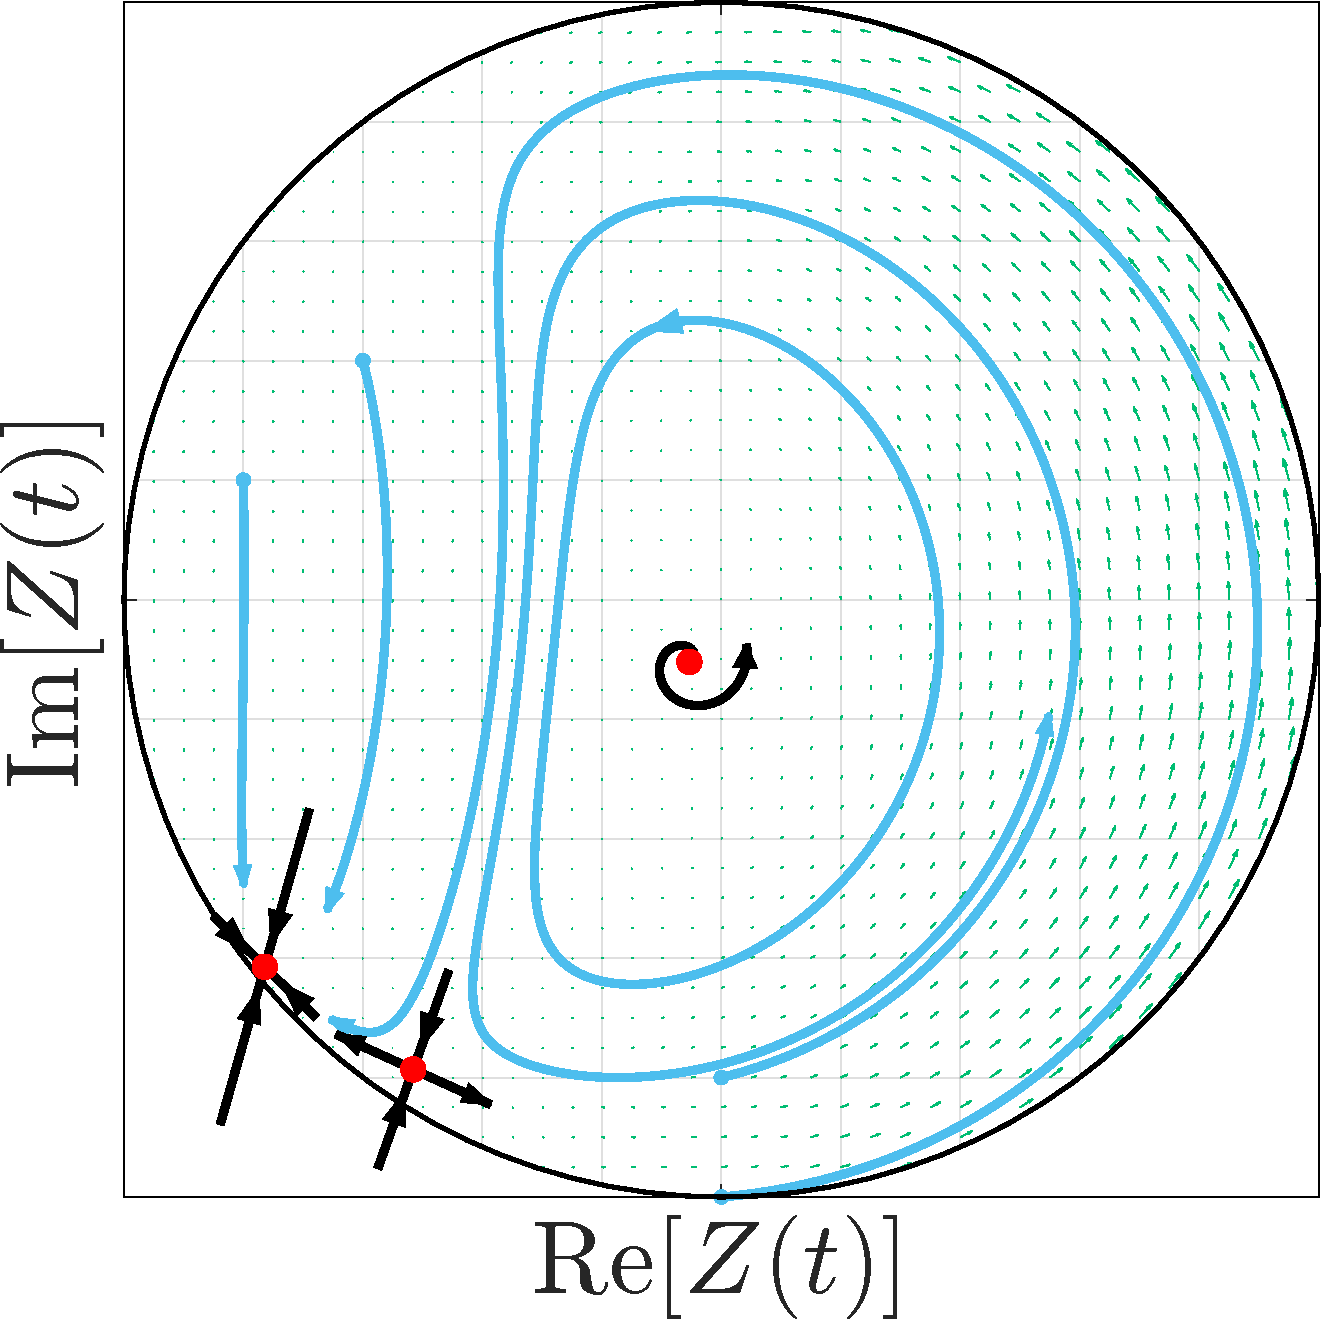
\includegraphics[width=\linewidth]{../Figures/PhaseSpace/MFRCPW.pdf}
   \caption{CPW state for $\eta_0 = 10.75, \sigma = 0.5$ and $\kappa= -9$. The mean field settles onto a stable limit cycle.}
   \label{fig:MFRCPW}
\end{subfigure}
   \caption{Three macroscopic states observed in the \MFR inside the imaginary unit circle $|Z(t)| = 1$. Green arrows mark the phase space vector field and blue trails mark solution curves. Red points indicate equilibrium points, with black arrows marking the direction of the eigenvectors in that point, scaled according to the magnitude of the corresponding eigenvalues. This information is found from the Jacobian, which we will discuss in Chapter \ref{sec:MFRSUndirected}.}
   \label{fig:macroscopicstatesfixeddegree}
\end{figure}


\subsection{Implications and challenges of the \MFR}
The advantages of using the \MFR can be found in the number of equations we now have left to investigate. As there are $M_{\k}$ equations in \eqref{eq:OttAntonsenSystemFull}, instead of $N$ equations for $N$ neurons, the reduction becomes more and more efficient for larger networks. As we have seen in \eqref{eq:MeanField} this yields a single equation for a fixed-degree network, as all neurons have the same degree.\\

While the \MFR gives us the opportunity to use any arbitray univariate distribution $P(k)$ for undirected, symmetric networks or any bivariate distribution $P(\k)$ for directed, asymmetric networks, none of the publications on the \MFR have treated directed networks. The challenge there is that the support $\K$ is a much larger set, as $\K = \koutb \times \kinb$. For example, the scale-free distribution \eqref{eq:scalefreepdf} has $M_{\k} = \kmax - \kmin$ number of degrees in its support. An example would be $M_{\k} = $ 1250, \cite{OttAntonsen2017}. For 10.000 neurons, that is a reduction of 87,5\%. When we wish to extend \eqref{eq:scalefreepdf} to a bivariate distribution, $M_{\k}$ grows to $\left( \kmax - \kmin \right)^2$. A bivariate distribution would therefore need about $1.56 \times 10^6$ equations for 10.000 neurons. It is not feasible to solve this many equations at once. Even though it is reported that solving only 10\% of the equations and then interpolation across $z$ and $t$ yields a very good approximation of the whole system, \cite{OttAntonsen2017}, the sheer number of equations remains high.

